\chapter{Cryptography and Distributed Ledgers Background}\label{ch:crypto-background}

This chapter is dedicated to background on cryptography primitives and distributed ledgers.
While such concepts are not required to understand the semantics or the implementation of Confis, they are helpful to understand blockchain-based smart contracts (an application of the original concept by Szabo~\cite{szabo1997smart-contracts}) which are discussed in~\autoref{sec:ethereum} and are a significant part of the state of the art when it comes to machine-readable of agreements between parties -- which does concern this project.


\section{Cryptography Primitives}\label{sec:cryptography}

\subsection{Hash Functions}\label{subsec:crypto:hash}

Hash functions are cryptographic functions designed to behave like random
functions~\cite{smart2016randomOracleModel}.
When building a security proof, they can be assumed to have the following properties~\cite{smart2016randomOracleModel,
    smart2016hashFunctions}:
% FIXME needs references
\begin{description}
    \item[Determinism] A hash function always produces the same output for the same input
    \item[One-way] It is computationally impossible to compute the preimage for some output of a hash function
    \item[Uniformity] Outputs of a hash function are expected to be uniformly distributed.
    In practice, the output space of a hash function is finite, so \textit{collisions} (where two inputs produce the
    same output) are possible, but uniformity ensures this is an unlikely scenario.
\end{description}

\subsection{Public Key Cryptography}\label{subsec:crypto:pubkey}

In public key cryptography, two communicating parties (say Alice and Bob) can communicate privately by using pairs of
numbers that are related mathematically and which allow converting cleartext into cyphertext and
back~\cite{smart2016publicKey}.
This pair of numbers is called an asymmetric keypair, and is composed of a \textbf{public key} $e$ and a \textbf{private
key} $d$.

In this example, if Alice wishes to communicate with Bob, Bob can generate a keypair $(d, e)$ and publish $e$.
Alice can then encrypt her cleartext with $e$, and only Bob will be able to decrypt it (because only Bob knows $d$).


Conversely, the same keypair can be used by Bob to send a message to Alice where Alice can verify that only Bob
could have written the message.
This is called \textit{signing}~\cite{smart2016signatures} and, more generally, it allows a sender of a message to
prove they are the authors of the message to a recipient.

\subsection{Secure Digital Timestamps}\label{subsec:crypto:timestamps}
% TODO citation for definiton
\textit{Trusted (digital) timestamping} is the process of securely proving that a document (for our purposes, a blob of
bytes) was created, was modified at, or existed at a certain point in time.
% TODO citation for widely used
In industry this is commonly implemented by trusting a Time Stamping Authority (TSA)~\cite{timestamps_tsp_rfc} that
signs (see~\nameref{subsec:crypto:pubkey}) a concatenation of the hash of the document and a timestamp representing some
time $t$.
Therefore, a party that trusts the TSA to provide the right timestamp can verify that, when the TSA made the signature,
the current time was $t$.

This method can be used for confidential data because the TSA does not perform the hashing of the original document
themselves - they are exposed only to its digest.

Additionally, the requester of the timestamp cannot deny they were not in possession of the original data at the time
% TODO verify statement
$t$ given by the timestamp, because it was them that produced its hash digest.

\subsubsection{Decentralised Timestamps}

Secure timestamps can also be achieved without relying on trusted parties by publishing the document digest to a
blockchain~\cite{gipp2015timestamps_btc}: blocks are public and cannot be tampered with (see~\nameref{subsec:btc:pow}),
so putting a signed digest in a block shows that the signer knew the original document at the time the block was
accepted by the network.


\section{Bitcoin Protocol}\label{sec:bitcoin}

Blockchain technology was introduced in~\cite{nakamoto2008bitcoin} as a decentralised system allowing for electronic
cash payments.
Blockchains are immutable distributed ledgers where participants' balances can be verified by every other participant,
and it is computationally hard to tamper with balances to perform attacks (such as performing a transaction where a
participant spends more funds than what they own).

I will provide a brief overview of how Bitcoin provides these guarantees.

\subsection{Transactions}\label{subsec:btc:txs}

\cite{nakamoto2008bitcoin} defines an \textit{electronic coin} as a chain of signatures: a payer can use their private
key, the hash of the previous transaction, and the payee's public key to create a signed hash that can be verified by
the payee (and used by them for \textit{their} next transaction).
This is illustrated in Figure~\ref{fig:bitcoin-tx}.

\begin{figure}[th]
    \centering
    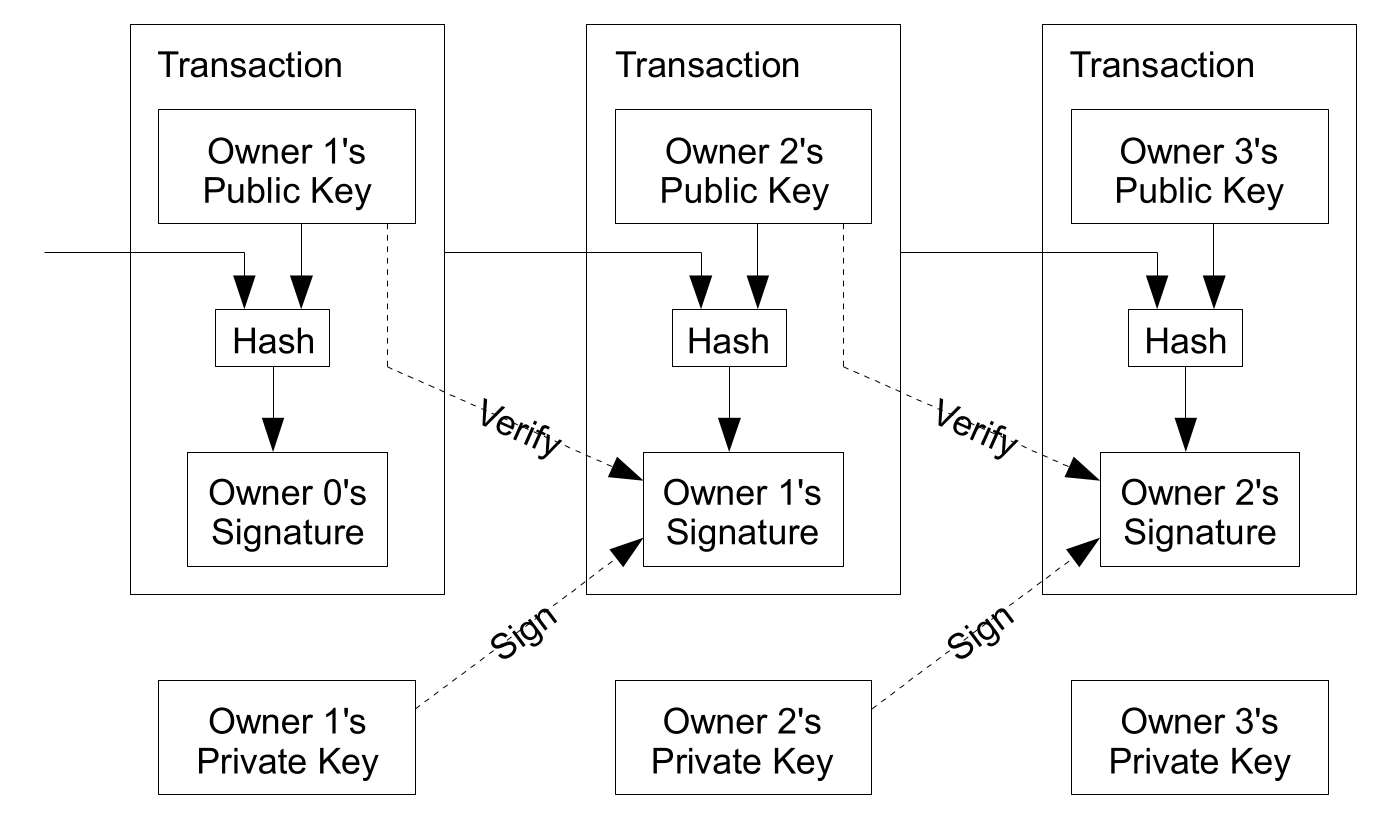
\includegraphics[width=0.8\columnwidth]{figures/bitcoin-tx}
    \caption[Bitcoin coin ownership transfer]{Transfer of ownership signature chain, from~\cite{nakamoto2008bitcoin}}
    \label{fig:bitcoin-tx}
\end{figure}

This ensures that, as long as a participants sign transactions at most once:
\begin{itemize}
    \item By verifying the chain of signatures, every participant can verify which participant owns which coin
    \item Only the owner of a coin can initiate a transaction with that coin
\end{itemize}

Bitcoin enforces that participants can only sign transactions once thanks to its proof-of-work
(see~\ref{subsec:btc:pow}) algorithm.

\subsection{Proof-Of-Work}\label{subsec:btc:pow}

Bitcoin ensures 'unique signatures' in transactions by grouping transactions in immutable, public \textit{blocks}.
Participants can then verify a payer has not signed a hash of a single transaction twice by looking at all existing
transactions.

Blocks are made immutable by including in them a value (called a \textit{nonce}) and the hash of the previous block.
% TODO verify it is the hash of the entire block that must yield the zeroes (implementation detail really)
The protocol then accepts only blocks where the $n$ first bits of its hash are zeroes. \\

Thus, in order to publish a block a participant must do work to find a nonce such that the block's hash meets this
condition - then other participants can verify its validity with a single hash operation.
This guarantees that a block cannot be changed (ie, a new copy published) without redoing the computational work.
Because blocks are chained (they include the hash of the previous block), in order to modify a transaction in the past
an adversary needs to redo the computational work for every block since that transaction (see Figure
\ref{fig:bitcoin-blockchain}).
% TODO implementation of mining rewards
Additionally, participants that successfully find a suitable nonce and propose new blocks (also referred to as
\textit{miners}) are allowed to add a specific transaction to the block where they own a newly created coin (also
referred to as \textit{mining reward}).

\begin{figure}[th]
    \centering
    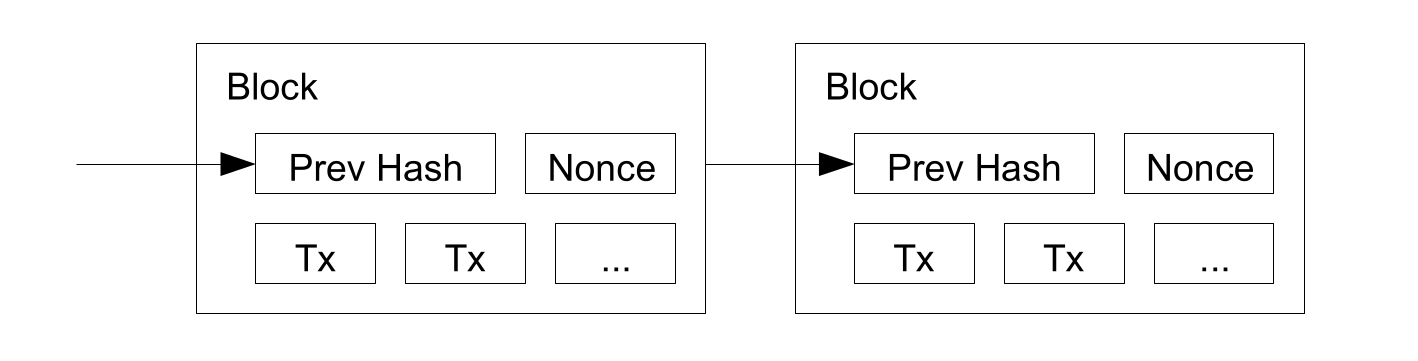
\includegraphics[width=0.8\columnwidth]{figures/bitcoin-blockchain}
    \caption[Two last blocks in a blockhain]{Two last blocks in a blockchain, from~\cite{nakamoto2008bitcoin}}
    \label{fig:bitcoin-blockchain}
\end{figure}

This model of consensus ensures that
\begin{itemize}
    \item Participants have a monetary incentive to stay honest with respect to the protocol
    \item An honest chain will out-compete an adversary's chain as long as the majority of computing power is honest
\end{itemize}

\subsection{Further details of the Bitcoin protocol}\label{subsec:btc.details}
\begin{figure}[th]
    \centering
    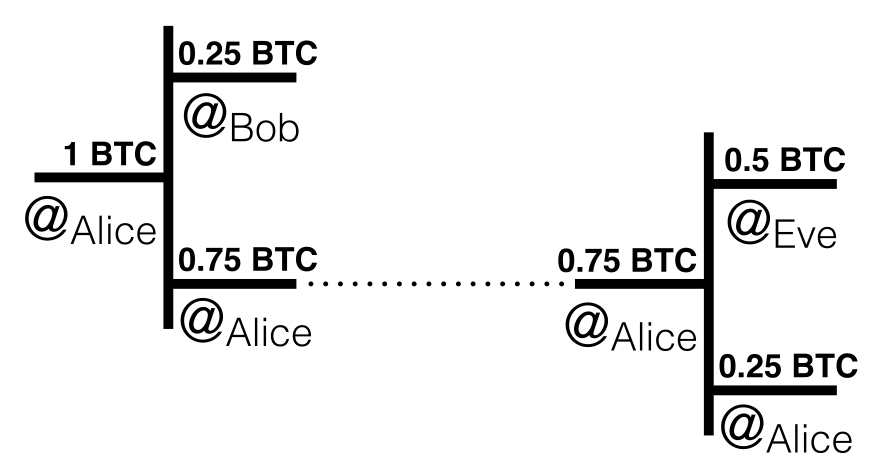
\includegraphics[width=0.6\columnwidth]{figures/bitcoin-2txs-outputs}
    \caption[Outputs and Inputs of two consecutive Transactions]{The outputs of a transaction correspond to
    the input of the next transaction (miner's fee not represented) from~\cite{gervais2022distribLedgers_transactionsInBitcoin}}
    \label{fig:bitcoin-2txs-outputs}
\end{figure}

While I provide a high-level overview of what makes the protocol function, there are many more details that combined
allow for more efficiency and usability:
\begin{itemize}
    \item Transactions may have several inputs and outputs, so participants can transfer amounts rather than single
    \textit{electronic coins}.
    When performing a payment, a typical transaction by Alice has two outputs: the amount she is paying Bob and the
    remainder, which makes up the rest of her funds (see Figure~\ref{fig:bitcoin-2txs-outputs}).
    Thus, a participant's balance is the sum of all the unspent outputs of previous transactions (the set of unspent
    outputs is commonly called the \textit{UTXO} set).
    \item By modifying how many of the leading bits of a blocks' hash must be zeroes, the average computation necessary
    to produce a new block can be adjusted by the protocol.
    \item By using Merkle Trees~\cite{merkle1980tree} transactions with fully spent transaction outputs can be discarded
    without breaking the block's hash.
    This allows compacting old blocks to reclaim disk space.
    \item A participant that does not wish to mine or hold a copy of the entire blockchain can still verify payments.
    It can keep a copy of the block headers of the longest chain and link a transaction to where it is on-chain and
    check that other network nodes have accepted it.
    This process is called \textit{Simple Payment Verification} (SPV)~\cite{nakamoto2008bitcoin}.
    \item Miners have an additional incentive (other than the mining reward) to verify transactions: the
    \textit{transaction fee}.
    The difference of the sum of a transaction's inputs and the sum its outputs corresponds to the transaction fee, which
    goes to the miner.
    \[
        \text{fee}_\text{miner} = \sum{\text{inputs}} - \sum{\text{outputs}}
    \]
    This provides an incentive for the miner to place this specific transaction in the block they propose.
\end{itemize}

For more information on all the workings of the Bitcoin protocol, please refer to~\cite{nakamoto2008bitcoin}.
